\chapter{Impedance and Sliding Mode Control of a One Degree of Freedom Exoskeleton}

\section{Exoskeleton Model}

\subsection{Exoskeleton}

In this study, we will use the upper limb exoskeleton described at chapter \ref{ch:ulexo}. It has one degree of freedom on the elbow joint, actuated by a DC motor with a Power Window Lifter gear transmission. The motor used is a 12V Mabuchi 578VA. The transmission has a 10:1 reduction ratio. The structure of the exoskeleton is constructed on aluminum. 

The exoskeleton is illustrated in figure \ref{exoskeleton system}. When the user tries to flex his arm, an electrical voltage can be recorded from the electrodes placed on the skin next to the biceps brachii. The SparkFun Muscle Sensor V3 was used to measure the EMG. It acquires the biceps muscle voltage, rectifies, low-pass filters  and amplifies the signal. This signal is sent to a microprocessor (in this case the ATmega328P), that makes the analog-to-digital conversion and applies a moving average filter. Finally the voltage signal is transformed into a desired joint angle. Equation \ref{eq:voltage_angle} shows the equation that gives the desired joint angle as a function of the EMG sensor voltage. A linear relationship between the angular position and the measured voltage was chosen. The equation was defined by measuring the lowest and highest voltage level acquired from the biceps muscle and linearly scaling it to the minimum angle of 0 and maximum angle of \(\frac{\pi}{2}\). It is important to note that the voltage from the EMG sensor is never zero. Even at a relaxed position, the sensor measures a residual voltage level.

\begin{equation}
\label{eq:voltage_angle}
\theta_d = -0.29 + 0.582 * V_{emg}
\end{equation}

\begin{figure}[thpb]
      \centering
      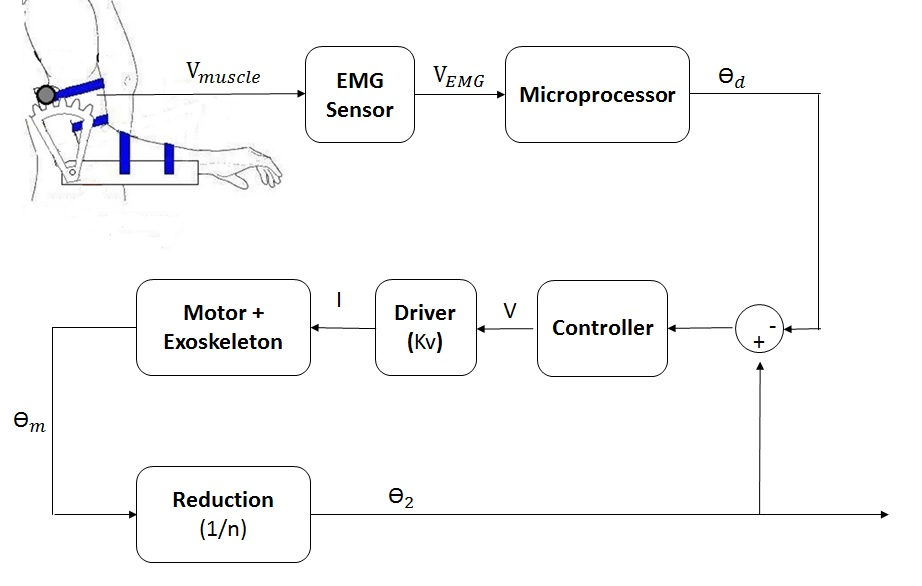
\includegraphics[scale=0.5]{Images/Exoskeleton_System.jpg}
      \caption{Diagram showing the exoskeleton block diagram control}
      \label{exoskeleton system}
   \end{figure}
   
   With the desired joint angle the PWM magnitude sent to the motor driver is calculated with a control logic in order to control the motor that actuates the exoskeleton. This control logic will be further studied in the next section. The motor driver input is the PWM voltage and its output is an electrical current. Equation \ref{eq:current} shows the relationship between PWM voltage and motor current:
   
   \begin{equation}
\label{eq:current}
I = K_v*V
\end{equation}

Where \(K_v = 1.42\) is the driver gain, V is the voltage applied to the driver and I is the output current of the driver.

The output electrical current from the driver goes to the motor, actuating the exoskeleton and consequently moving the user’s forearm.

\subsection{Modeling}

Even though the exoskeleton has only one degree of freedom on the elbow joint, the user's shoulder angle should be considered because it influences the forces applied to the exoskeleton and the arm. The exoskeleton can be modeled as two segments: the upper arm (between shoulder and elbow) and the forearm (between elbow and wrist).

\begin{figure}[thpb]
      \centering
      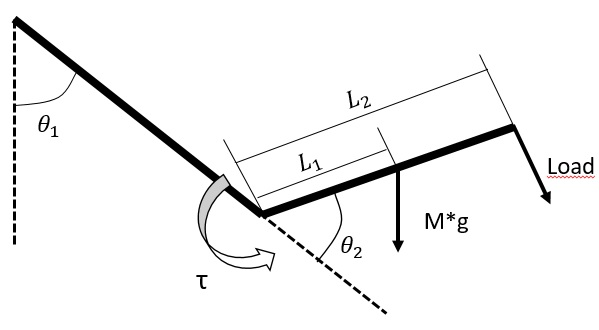
\includegraphics[scale=0.5]{Images/DCL_exoesqueleto.jpg}
      \caption{Free body diagram of the exoskeleton}
      \label{exoskeleton fbd}
   \end{figure}

Figure \ref{exoskeleton fbd} shows the exoskeleton free body diagram, where the upper arm is considered to be fixed at a given angle \(\theta_1\), \(\theta_2\) is the angle between the upper arm and the forearm with a motion range between 0 and \(\frac{\pi}{2}\) rad, \(\tau\) is the torque applied by the motor, the Load has a range between 0 and 100N, M is the sum of the human forearm and exoskeleton forearm masses that equals 2.14 kg, \(L_1\) is the distance between the elbow center and the forearm center of mass (0.12m), \(L_2\) is the length of the forearm (0.22m), \(J_e\) is the forearm moment of inertia \(5.6 \cdot 10^{-3}  kg\cdot m^2\).

Equation \ref{eq:coupled exo motor} shows the dynamics of the exoskeleton:

\begin{equation}
\label{eq:coupled exo motor}
\left(\frac{J_e}{n}+J_m\right)\cdot \ddot{\theta}_m+B \cdot \dot{\theta}_m = \tau + \frac{-L_2 \cdot Load - L_1 \cdot M \cdot g \cdot sin\left(\frac{\theta_m}{n}+\theta_1\right)}{n}
\end{equation}
   
   Equation \ref{eq:motor torque} gives the relation between motor input current and output torque:
   
   \begin{equation}
\label{eq:motor torque}
\tau = k_m \cdot I
\end{equation}

Using equations \ref{eq:current}, \ref{eq:coupled exo motor} and \ref{eq:motor torque} gives the exoskeleton and human dynamics:

\begin{equation}
\label{eq:plant dynamics}
\left(\frac{J_e}{n}+J_m\right)\cdot \ddot{\theta}_m+B \cdot \dot{\theta}_m = K_m \cdot K_v \cdot V +\frac{-L_2 \cdot Load - L_1 \cdot M \cdot g \cdot sin\left(\frac{\theta_m}{n}+\theta_1\right)}{n} 
\end{equation}

Where \(\theta_m\) is the angle of the shaft of the motor, \(J_m = 6 \cdot 10^{-5} kg \cdot m^2\) is the inertia of the motor, B = 1.2732 is the damping coefficient of the motor, n = 10 is the reduction factor and \(K_m = 0.533\) is the electrical current gain of the motor.

\section{Control}

\subsection{General Characteristics}

The action control will be the voltage V applied to the driver of the motor. 
The load applied to the exoskeleton can vary from 0N to 100N. In this way the user will be able to manipulate different objects without changing the control parameters in a short time span. The controller goal is to control the exoskeleton position while maintaining safety and confort. The range of motion of the elbow joint is from 0 to \(\frac{\pi}{2}\) rad while the maximum angular velocity must be around \(\frac{\pi}{4}\) rad/s. There must be no overshoot on the movement.

\subsection{Impedance Control}

The first law will be based on impedance control. Impedance control imposes a dynamic behavior to the interaction between the target system and the environment, usually a mass-spring-damper system.	
Impedance control is suited for tasks that require contact forces without an accurate control of the end-effector position (e.g. grabing an object). That is especially important in biomechanical applications since the human arm is capable of doing delicate tasks without a profound knowledge of necessary forces to be applied to the target objects. 
One drawback is that whenever an external force is applied on the system the final position of the end-effector will not necessarily be the desired one, instead it controls a combination of force and position. The chosen stiffness for the dynamic system will regulate this trade-off between contact force and position accuracy.

\subsection{Impedance Control Design}

The system dynamics, (equation \ref{eq:plant dynamics}), can be rewritten as follows:


\begin{equation}
\begin{split}
\label{eq:rewritten plant}
\ddot{\theta}_m = \frac{-B \cdot \dot{\theta}_m + \frac{-L_2 \cdot Load - L_1 \cdot M \cdot g \cdot sin (\frac{\theta_m}{n}+\theta_1 )}{n} + K_v \cdot K_m \cdot V }{\frac{J_e}{n}+J_m}
\end{split}
\end{equation}

Equation \ref{eq:rewritten plant} can be organized in the form:

\begin{equation}
\label{eq:reorg}
\ddot{\theta}_m = f + bu
\end{equation}

Where:

\begin{equation}
\label{eq:f}
f = \frac{-B \cdot \dot{\theta}_m + \frac{-L_2 \cdot Load - L_1 \cdot M \cdot g \cdot sin \left(\frac{\theta_m}{n}+\theta_1 \right)}{n}}{\frac{J_e}{n}+J_m}
\end{equation}

\begin{equation}
\label{eq:b}
b = \frac{K_v \cdot K_m}{\frac{J_e}{n}+J_m}
\end{equation}

\begin{equation}
\label{eq:u}
u = V
\end{equation}

The desired closed loop dynamics are:

\begin{equation}
\label{eq:desired}
M_d \cdot (\ddot{\theta}_m-\ddot{\theta}_d) + B_d \cdot (\dot{\theta}_m - \dot{\theta}_d) + K_d \cdot (\theta_m - \theta_d) = -F
\end{equation}

Where \(M_d\) is the desired inertia, \(B_d\) is the desired damping, \(K_d\) is the desired stiffness, \(\theta_d\) is desired position and 

\begin{equation}
\label{eq:F}
F = \frac{L_2 \cdot Load}{n}
\end{equation}

This characterizes a mass-spring-damper dynamics that will be imposed to the system by the controller.

By substituting equation \ref{eq:desired} in equation \ref{eq:reorg} and rearranging, one gets:

\begin{equation}
\label{eq:subs1}
u = b^{-1} \left(-f+ \frac{M_d \cdot \ddot{\theta}_d-B_d \cdot (\dot{\theta}_m-\dot{\theta}_d)-K_d \cdot (\theta_m-\theta_d)-F}{M_d}\right)
\end{equation}

Equation \ref{eq:subs1} gives the control law for the system, that can be expressed as (using \ref{eq:rewritten plant} - \ref{eq:F})

\begin{equation}
\begin{split}
\label{eq:inpedance law}
V = {} & \frac{1}{K_v \cdot K_m} (B \cdot \dot{\theta}_m + \frac{L_2 \cdot Load}{n} + \frac{L_1 \cdot M \cdot g \cdot sin(\frac{\theta_m}{n}+\theta_1)}{n} + \\ 
& (\frac{J_e}{n}+J_m)(M_d \cdot \ddot{\theta}_d - B_d(\dot{\theta}_m-\dot{\theta}_d)-K_d(\theta_m-\theta_d)-\frac{L_2 \cdot Load}{n})\cdot \frac{1}{M_d})
\end{split}
\end{equation}

This control law, as it is presented, cancels the nonlinearities of the system and imposes the desired dynamic  system behavior to the exoskeleton.

\subsection{Sliding Mode Control Design}

The second applied control law will be the Sliding Mode control. The system dynamics are the same as shown in equation \ref{eq:coupled exo motor}

The desired sliding surface is:

\begin{equation}
\label{eq:SM}
s = \dot{\theta}_m - \dot{\theta}_{d} + \lambda \cdot (\theta_m-\theta_{d})
\end{equation}

The control signal is u and, to achieve the desired controlled dynamics of the system, its value is as follows:

\begin{equation}
\label{eq:uSM}
u = \hat{b}^{-1}\left(-\hat{f}+\ddot{\theta}_{d} -\lambda \cdot (\theta_m-\theta_{d})-K\cdot sat\left(\frac{s}{\phi}\right)\right)
\end{equation}

Where:

\begin{equation}
\label{eq:bSM}
\hat{b} = \frac{K_v \cdot K_m}{\frac{J_e}{n}+\hat{J}_m}
\end{equation}

\begin{equation}
\label{eq:fSM}
\hat{f} = \frac{-B \cdot \dot{\theta}_m + \frac{-L_2 \cdot \hat{Load} - L_1 \cdot M \cdot g \cdot sin(\frac{\theta_m}{n}+\theta_1)}{n}}{\frac{J_e}{n}+\hat{J}_m}
\end{equation}

\(\hat{J_m}\) is the motor inertia with measuring error and \(\hat{Load}\) is the external load applied to the exoskeleton with measuring error.

This way, when in closed loop, the system acquires the following dynamics:

\begin{equation}
\label{eq:CLSM}
\frac{ds}{dt} = (\ddot{\theta}_m-\ddot{\theta}_{d})+\lambda \cdot (\dot{\theta}_m-\dot{\theta}_{d})
\end{equation}

That is,

\begin{equation}
\begin{split}
\label{eq:CLSM}
\frac{ds}{dt} = {} & f + b \cdot \hat{b}^{-1} \cdot (-\hat{f}) + b \cdot \hat{b}^{-1} \cdot (\ddot{\theta}_{d} - \lambda \cdot (\theta_m - \theta_{d}) +  \\
& - b \cdot \hat{b}^{-1} \cdot K \cdot sat(\frac{s}{\phi})-\ddot{\theta_m} + \lambda \cdot (\dot{\theta}_m-\dot{\theta}_{d}))
\end{split}
\end{equation}

To guarantee convergence the control must satisfy a sliding condition:

\begin{equation}
\label{eq:condition}
\frac{1}{2}\frac{ds^2}{dt} \leq -\eta \cdot |s|
\end{equation}

Equation \ref{eq:condition}, using \ref{eq:CLSM}:

\begin{equation}
\label{eq:K}
K \leq \beta \cdot (\eta + F) + (\beta -1) \cdot |\hat{u}|
\end{equation}

Where,
\begin{equation}
\label{eq:beta}
\beta = \sqrt{\frac{b_{max}}{b_{min}}}
\end{equation}

\begin{equation}
\label{eq:Fsm}
F > |f-\hat{f}|
\end{equation}

\begin{equation}
\label{eq:uhat}
\hat{u} = -\hat{f} + \ddot{\theta}_{d}-\lambda \cdot (\theta_m - \theta_{d})
\end{equation}

\section{Results}

\subsection{Impedance Control}

Choosing \(M_d = 1 kg \cdot m^2, B_d = 4 N \cdot m \cdot s, K = 4.5 N \cdot m\) and \(\theta_d = 1 rad\) gives \(\omega_n = \frac{2\pi}{8}\) rad/s the natural frequency of the system, \(t_{0-90\%} = 2.4 s\) the time the system takes to reach 90\% of the final position and \(\zeta > 1\) the damping factor, since there must be no overshoot.

Figures \ref{posicao0} and \ref{posicao100} show the results of a simulation where \(\theta_d = 1 rad\) and external load = 0 and 100N, respectively.

\begin{figure}[thpb]
      \centering
      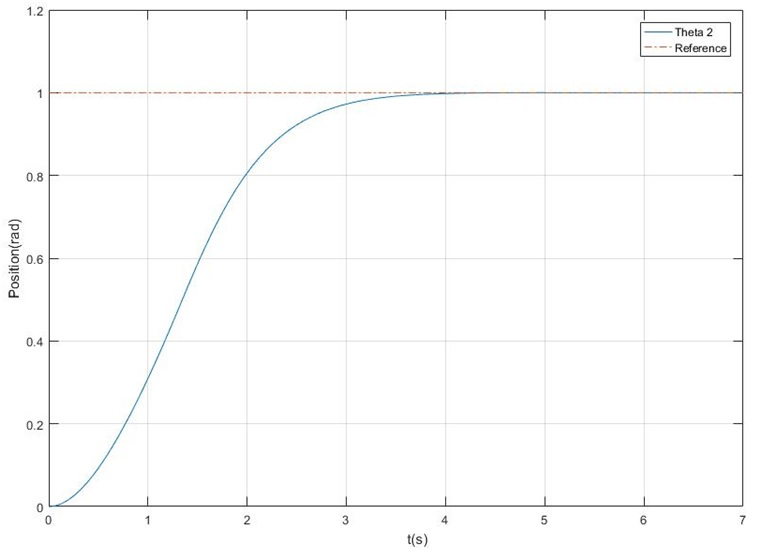
\includegraphics[scale=0.5]{Images/posicao_load_0_paper.jpg}
      \caption{Position \(\theta_2\) versus time for an external load = 0}
      \label{posicao0}
   \end{figure}
   
   \begin{figure}[thpb]
      \centering
      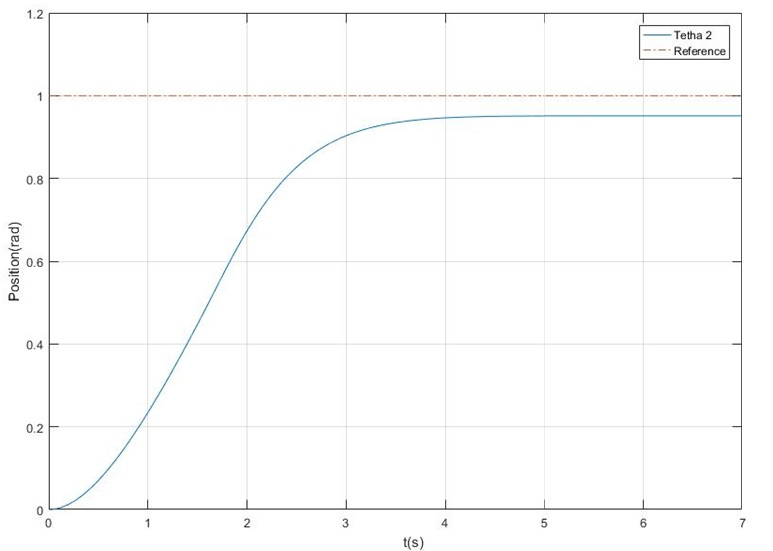
\includegraphics[scale=0.5]{Images/posicao_load_100_paper.jpg}
      \caption{Position \(\theta_2\) versus time for an external load = 100 N}
      \label{posicao100}
   \end{figure}

\subsection{Sliding Mode Control}

Considering the measured load with 30\% error and the measured motor inertia with 20\% error, that is, \(\hat{Load} = 130N\) and \(\hat{J}_m = 7.2 \cdot 10^{-5} kg \cdot m^2\), resulting in \(\beta = 1.04\), the system was simulated with the following parameters: \(\eta = 5, \lambda = 1\) and \(\phi = 10\) and the results for the position and the sliding surface can be found in figures \ref{posicaoSliding} and \ref{slidingSurface}, respectively.

\begin{figure}[thpb]
      \centering
      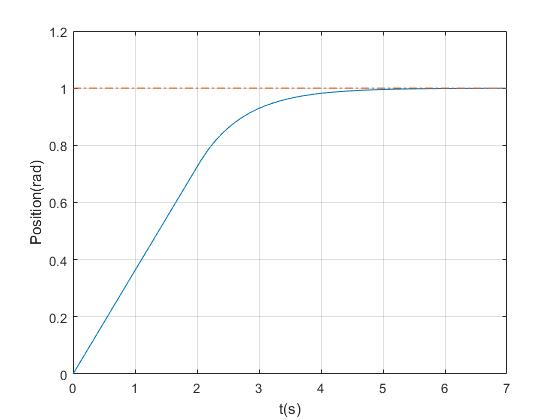
\includegraphics[scale=0.5]{Images/Sliding_mode_position.jpg}
      \caption{Position \(\theta_2\) versus time}
      \label{posicaoSliding}
   \end{figure}
   
   \begin{figure}[thpb]
      \centering
      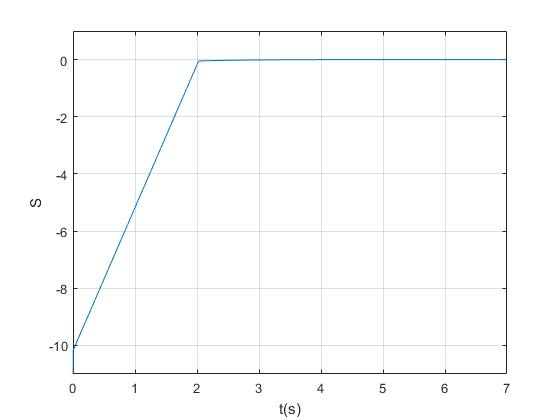
\includegraphics[scale=0.5]{Images/Sliding_mode_S.jpg}
      \caption{Sliding surface versus time}
      \label{slidingSurface}
   \end{figure}

\section{Conclusions}

Both control approaches has advantages and drawbacks. The impedance control cannot reach a desired position with utmost accuracy since the external load, by definition, will take the system out of its desired final position and the system parameters must be precisely measured in order to guarantee accurate desired dynamics. On the other hand, precise activities can be achieved without a deep knowledge of the environment, the system acquires familiar characteristics in the form of a mass-spring-dampener system and it is safer for the user since the controller changes the position of the system when an excessive external load is detected. The sliding mode control can achieve great precision and accuracy of desired position and trajectory and does not require a precise measurement of the system characteristics.

Depending on the application each one of these control methods is more appropriated. In the case of a wearable exoskeleton, the impedance control is a more suitable control method, since it offers a dynamic behavior close to that of a human limb and is safer for the user. To control an external robotic arm, the sliding mode control can be used since it will cause no harm to the user and is capable of performing actions with higher accuracy.